\documentclass[a4paper, 11pt, twocolumn]{article}
\usepackage[left=1.5cm, top=2.5cm, total={18cm, 25cm}]{geometry}
\usepackage[utf8]{inputenc}
\usepackage[slovak]{babel}
\usepackage[T1]{fontenc}
\usepackage[unicode, hidelinks]{hyperref}
\usepackage{graphicx}
\usepackage[nottoc]{tocbibind}
\usepackage{url}
\usepackage[square,numbers]{natbib}

\begin{document}

\begin{titlepage}
    \begin{center}
        \Huge
        \textsc{Fakulta informačních technologií \\
        Vysoké učení technické v Brně} \\
        \vspace{\stretch{0.382}}
        
        \LARGE
        Počítačové komunikácie a~siete -- 2.~projekt \\
        Variant ZETA: Sniffer paketov \\
        \vspace{\stretch{0.618}}
    \end{center}
    
    {\Large 2021 \hfill
    Jakub Bartko (xbartk07)}
\end{titlepage}

\onecolumn
\tableofcontents
\twocolumn

\section{Úvod}
    Táto dokumentácia má za účel poskytnúť základný prehľad o~riešenom probléme, implementácií jeho riešenia, využívaných knižniciach a~o~už existujúcich prostriedkoch s~obdobným využitím.

\section{Základná problematika}
    Centrálnym prvkom projektu, ku ktorému táto dokumentácia náleží, je \textbf{analyzátor paketov} (angl. aj \textit{packet sniffer}). Takýto program alebo zariadenie skúži na sledovanie, zachytávanie a~zaznamenávanie sieťovej prevádzky na určitej digitálnej sieti (preložené z~\cite{packetanalyzer}). V~tomto projekte je využívaný na nájdenie aktívnych sieťových rozhraní a~zachytávanie, filtrovanie a~základnú analýzu paketov na konkrétnom rozhraní.
    
    \textbf{Sieťové rozhranie} je prepojenie medzi počítačom a~súkromnou alebo verejnou sieťou (preložené z~\cite{networkinterface}). \textbf{Paket} je malý blok dát prenášaný v~sieti, ktorý sa skladá z~hlavičky a~samotných prenášaných dát. Táto hlavička obsahuje informácie, ako napr. zdrojovú a~cieľovú adresu paketu, jeho veľkosť a~použitý protokol. \textbf{Protokol} definuje formát dát paketu, t.~j.~stanovuje, na ktorých bajtoch sa nachádzajú určité informácie. Každá z~vrstiev modelu OSI (abstraktná štruktúra komunikačných a~počítačových sieťových protokolov \cite{osi}) má vlastný balík protokolov. Paket môže obsahovať viacero hlavičiek protokolov na rôznych vrstvách v~súlade s tým, pod ktorú vrstvu spadá. My, na základe zadania, začneme od ethernetového rámca, z~ktorého hlavičky zistíme, ktorý protokol sieťovej vrstvy bol použitý, t.~j.~aký formát ďalšej hlavičky máme očakávať. Z~týchto hlavičiek potom zistíme, či na výstupe máme zahrnúť IPv4, IPv6 alebo MAC adresu, prípadne port, rovnako ako to, na ktorých bajtoch tieto informácie nájdeme.
    
    Na analýzu paketov budeme využívať \textbf{promiskuitný režim} sieťovej karty, čo znamená, že budeme zachytávať aj sieťovú komunikáciu, ktorá nie je priamo určená našemu zariadeniu \cite{promisc}.


\section{Štruktúra kódu a~implementácia}
    Funkcionalitu programu \texttt{ipk-sniffer} je v~základe možné rozdeliť na spracovanie argumentov príkazového riadka, výpis dostupných sieťových rozhraní a~zachytávanie a~analýzu paketov na zvolenom rozhraní. Na základné operácie s~rozhraniami a~paketmi sa využíva knižnica \texttt{pcap}\footnote{\href{https://www.tcpdump.org/manpages/pcap.3pcap.html}{https://www.tcpdump.org/manpages/pcap.3pcap.html}}.
    
    Na základe argumentov príkazového riadka, spracovaných pomocou štandardnej knižnice \texttt{getopt}\footnote{\href{https://man7.org/linux/man-pages/man3/getopt.3.html}{https://man7.org/linux/man-pages/man3/getopt.3.html}}, sa zvolí činnosť analyzátora\,--\,výpis rozhraní alebo analýza paketov, a~zostaví sa filter na ich zachytávanie. Tieto argumenty, spracované funkciou \texttt{Options::get\_opts}, sú uložené v~objekte triedy \texttt{Options}. Zoznam názvov dostupných rozhraní sa získa pomocou funkcie \texttt{pcap\_findalldevs}. Tento zoznam sa následne iteruje, názvy rozhraní sa vypíšu na štandardný výstup a~zoznam sa uvoľní.
    
    V~prípade analýzy paketov sa najskôr získa \uv{rukoväť} (ďalej angl. \textit{handle}) v~promiskuitnom móde na zachytávanie paketov na špecifikovanom sieťovom rozhraní a~vygeneruje, skompiluje a~aplikuje sa na ňu filter na základe údajov objektu triedy \texttt{Options}. Následne sa zachytí a~spracuje zvolený počet paketov.
    
    Z~hlavičky zachyteného paketu sa získa časová značka a~jeho veľkosť v~bajtoch. Tento paket sa interpretuje ako ethernetový rámec a~na základe hodnoty atribútu \texttt{EtherType}\footnote{\href{https://en.wikipedia.org/wiki/Ethernet\_frame\#Types}{https://en.wikipedia.org/wiki/Ethernet\_frame\#Types}} sa zistí, či obsahuje IPv4 datagram alebo rámec IPv6 či ARP a získa sa príslušná hlavička. V~prípade IPv4 alebo IPv6 sa získa a~dekóduje zdrojová a~cieľová IP adresa paketu a pri protokoloch TCP a UDP aj príslušná dvojica portov; v~prípade ARP sa z~hlavičky ethernetového paketu zistí dvojica MAC adries. Údaje popísané v~tomto odstavci sa vypíšu na štandardný výstup ako hlavička výpisu zachyteného paketu.
    
    Samotné dáta zachyteného paketu sú po 16 bajtoch na riadok vypísané ako hexadecimálne hodnoty spolu so svojou ASCII reprezentáciou. Prefix každého riadka predstavuje hexadecimálny ofset jeho prvého bajtu.

\section{Testovanie funkcionality}
    Priebežné testovanie implementovaného programu bolo vykonávané za použitia open-source analyzátora paketov \textbf{Wireshark 3.2.3} \cite{ws}. Finálne testovanie pozostávalo z~niekoľkých testovacích prípadov, ktoré zahŕňali spustenie oboch nástrojov, lokalizáciu zaujímavého úseku paketov, vyexportovanie skúmaných dát a~ich porovnanie.
    \pagebreak
    \begin{figure}[h]
        \centering
        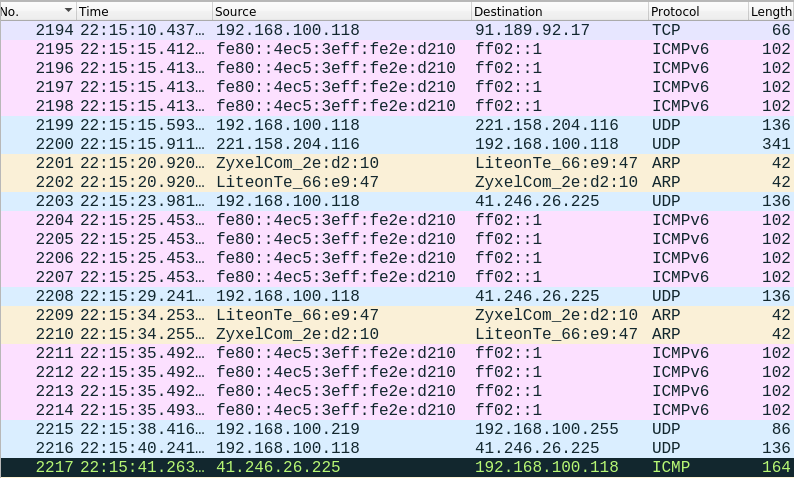
\includegraphics[width=0.48\textwidth]{img/ws1.png}
        \caption{Skúmaný úsek paketov\,--\,\textit{Wireshark}}
    \end{figure}    
    \begin{figure}[h]
        \centering
        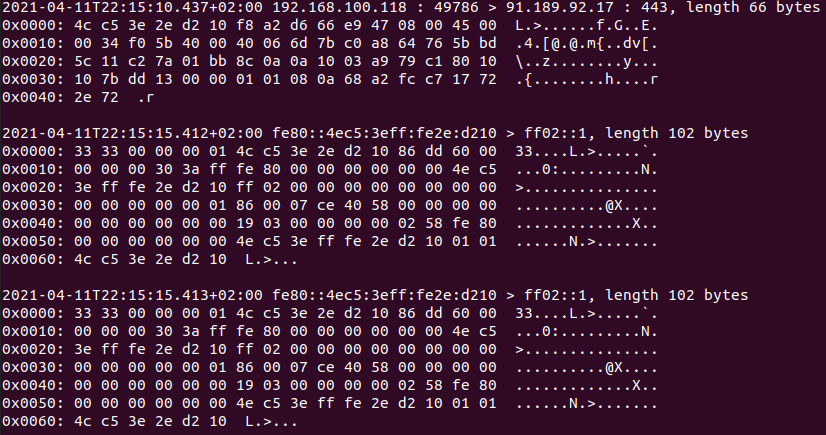
\includegraphics[width=0.48\textwidth]{img/my1.png}
        \caption{Časť skúmaného úseku paketov\,--\,\textit{ipk-sniffer}}
    \end{figure} 
    
    \subsection{Správnosť zachytávania paketov}
        Prvý testovací prípad skúma, či implementovaný analyzátor zachytáva rovnaké pakety. Zvolíme si prvé 4~pakety skúmaného úseku a~porovnáme ich časovú značku a~veľkosť. \textit{WS}\,--\,Wireshark, \textit{IPK}\,--\,ipk-sniffer.
        
        \begin{table}[h]
            \centering
            \scalebox{0.75}{
                \begin{tabular}{|c|c||c|c|}
                    \hline
                    WS čas & IPK čas & WS veľkosť & IPK veľkosť\\ \hline
                    22:15:10.437 & 22:15:15.437+02:00 & 66 & 66\\ \hline
                    22:15:15.412 & 22:15:15.412+02:00 & 102 & 102\\ \hline
                    22:15:15.413 & 22:15:15.413+02:00 & 102 & 102\\ \hline
                    22:15:15.413 & 22:15:15.413+02:00 & 102 & 102\\ \hline
                \end{tabular}
            }
            \caption{Porovnanie zachytených paketov}
        \end{table}
        
        Zdá sa, že obidva analyzátory zachytávajú rovnaké pakety. Ďalej teda budeme testovať ich obsah.
        
    \subsection{Správnosť obsahu paketov}
        V~rámci tohoto testovacieho prípadu si zvolíme niekoľko paketov zo skúmaného úseku s~rôznymi protokolmi a~porovnáme ich obsahy v~hexadecimálnej aj ASCII reprezentácií. \\
        
        \begin{figure}[ht]
            \centering
            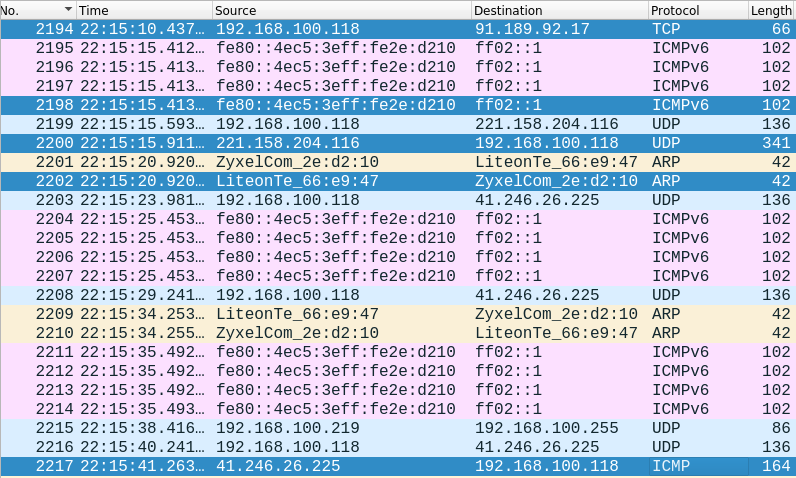
\includegraphics[width=0.48\textwidth]{img/ws2.png}
            \caption{Zvolené pakety (tmavo modré)\,--\,\textit{Wireshark}}
        \end{figure}
        
        Porovania boli vykonané príkazom\texttt{\footnote{\texttt{wdiff}\,--\,GNU nástroj na porovnávanie súborov po slovách; \texttt{colordiff}\,--\,\href{https://linux.die.net/man/1/colordiff}{https://linux.die.net/man/1/colordiff}}} \texttt{wdiff \{protocol\} \{protocol\}\_ws | colordiff}. Z~výsledkov tohoto testovacieho prípadu na obr.~\ref{fig:fig1}~a~\ref{fig:fig2}~vidíme, že výstup programu \textit{ipk-sniffer} sa od dát zachytených programom \textit{Wireshark} líši jedine vo výpise hlavičky a~vo formáte ofsetu na začiatku riadku.
        
        \begin{figure}[hb]
            \centering
            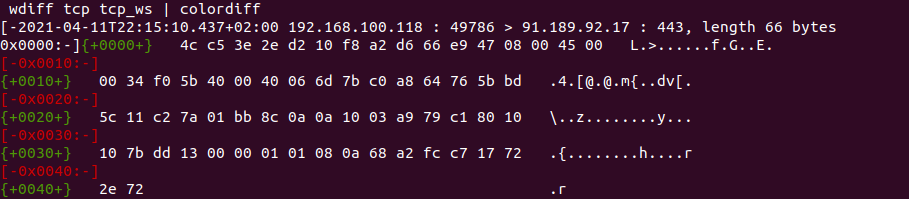
\includegraphics[width=0.48\textwidth]{img/tcp.png}
            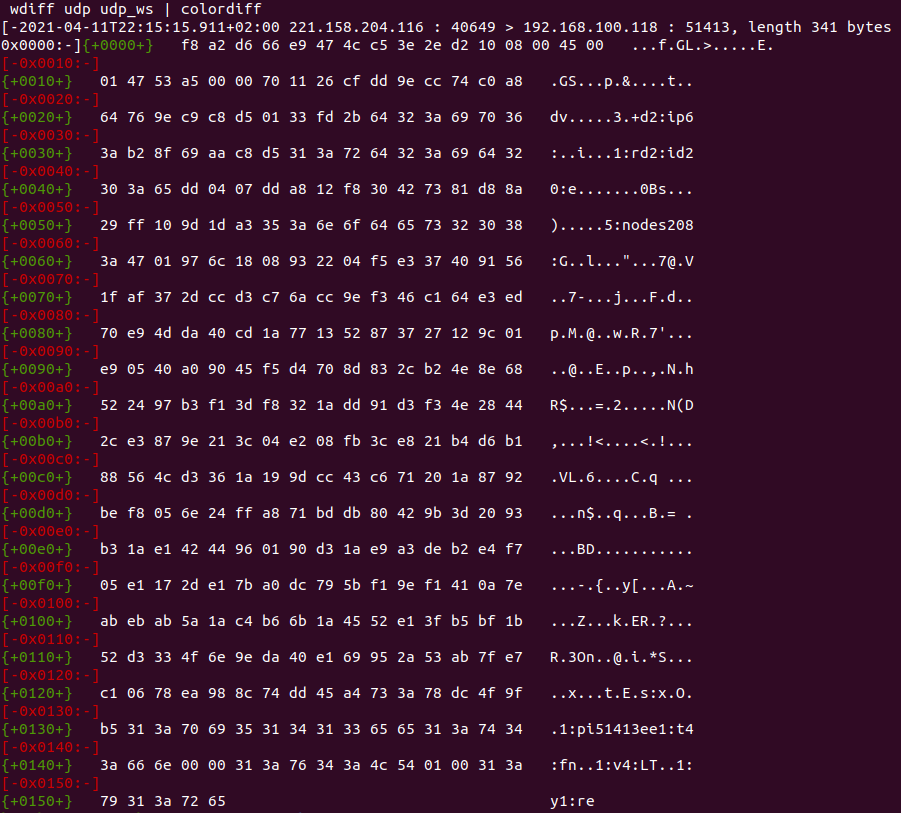
\includegraphics[width=0.48\textwidth]{img/udp.png}
            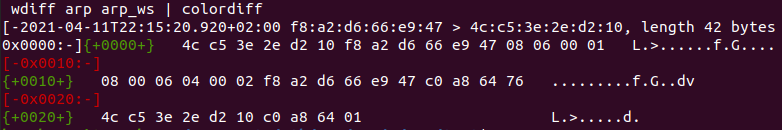
\includegraphics[width=0.48\textwidth]{img/arp.png}
            \caption{Výsledky porovnávania dát paketov\,--\,1.~časť}
            \label{fig:fig1}
        \end{figure}
        \begin{figure}[ht]
            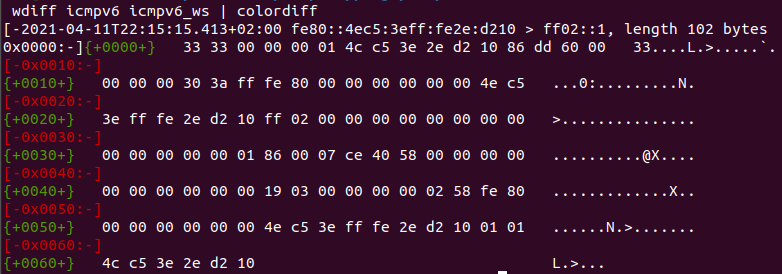
\includegraphics[width=0.48\textwidth]{img/icmpv6.png}
            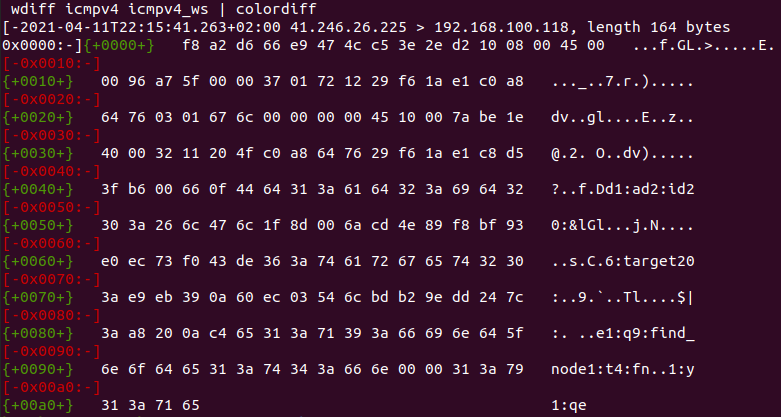
\includegraphics[width=0.48\textwidth]{img/icmpv4.png}
            \caption{Výsledky porovnávania dát paketov\,--\,2.~časť}
            \label{fig:fig2}
        \end{figure}
        
\bibliography{citations}
\bibliographystyle{abbrvnat}

\end{document}
